% !TeX program = xelatex
% Compile from the project root: xelatex -output-directory=presentations/tex presentations/tex/SEA_2026.tex
% Built from the AHEW 2026 summary frames (conferences/ahew-2026/slides/main.tex); numbers come
% from the paper's macro files, figures from results/figures/.
\documentclass[aspectratio=169,11pt]{beamer}

\usepackage{graphicx}
\usepackage{booktabs}
\usepackage{array}
\usepackage{tikz}
\usetikzlibrary{positioning, arrows.meta}
\usepackage{hyperref}
\usepackage{amsmath}

\usepackage{presentations/tex/theme/beamerthemeResearch}

%% Auto-generated by A1-desc-stats.do — do not edit by hand
\newcommand{\nPCPs}{51,702}
\newcommand{\nSpecialists}{18,912}
\newcommand{\meanRefsPerPCP}{4.7}
\newcommand{\meanSpecsPerPCP}{3.4}
\newcommand{\meanRefsPerPair}{1.4}
\newcommand{\meanFailuresPerPCP}{0.5}
\newcommand{\failureRateMean}{9}
\newcommand{\specFailurePtwentyfive}{4.7}
\newcommand{\specFailurePseventyfive}{15.4}
\newcommand{\failureIQRPtwentyfive}{5.5}
\newcommand{\failureIQRMedian}{6.3}
\newcommand{\failureIQRPseventyfive}{7.1}
\newcommand{\paymentIQRMedian}{8}
\newcommand{\capacitySuffPct}{50}
\newcommand{\meanChoiceSet}{176}
\newcommand{\meanSpecsPerHRR}{292}
\newcommand{\runningReferrals}{4.1}
\newcommand{\specsPerHRRYear}{70}
\newcommand{\cumlNetworkSize}{10}
\newcommand{\nHRRsMNL}{296}

%% Auto-generated by O2-structural-summary.do — do not edit by hand
\newcommand{\reallocationMeanMyopic}{39.6}
\newcommand{\healthFXMeanMyopic}{0.5}
\newcommand{\nHRRsMyopic}{280}
\newcommand{\nAlphaZeroMyopic}{51}
\newcommand{\alphaDistRatioMyopic}{2.9}
\newcommand{\nHRRsEtaFiveMyopic}{281}
\newcommand{\reallocationMeanFullFamMyopic}{40.0}
\newcommand{\healthFXMeanFullFamMyopic}{0.4}
\newcommand{\partialFXNonzeroMyopic}{3.4}
\newcommand{\partialFXAllMyopic}{2.5}
\newcommand{\reallocationMeanFWD}{32.1}
\newcommand{\healthFXMeanFWD}{0.4}
\newcommand{\nHRRsFWD}{277}
\newcommand{\nAlphaZeroFWD}{46}
\newcommand{\alphaDistRatioFWD}{3.8}
\newcommand{\nHRRsEtaFiveFWD}{279}
\newcommand{\reallocationMeanFullFamFWD}{35.0}
\newcommand{\healthFXMeanFullFamFWD}{0.4}
\newcommand{\partialFXNonzeroFWD}{3.0}
\newcommand{\partialFXAllFWD}{2.0}

%% Auto-generated by A2b-rereferral.do
\newcommand{\rereferEvents}{1190521}
\newcommand{\rereferFailures}{112871}
\newcommand{\rereferBase}{0.160}
\newcommand{\rereferFX}{-0.0110}
\newcommand{\rereferSE}{0.0011}
\newcommand{\rereferPct}{-6.8}
\newcommand{\rereferFXpcp}{-0.0106}
\newcommand{\rereferSEpcp}{0.0011}
\newcommand{\rereferFXhistzero}{-0.0126}
\newcommand{\rereferSEhistzero}{0.0013}
\newcommand{\rereferBasehistzero}{0.059}
\newcommand{\rereferPcthistzero}{-21.2}
\newcommand{\rereferFXhistone}{-0.0100}
\newcommand{\rereferSEhistone}{0.0018}
\newcommand{\rereferBasehistone}{0.131}
\newcommand{\rereferPcthistone}{-7.6}
\newcommand{\rereferFXhisttwo}{-0.0093}
\newcommand{\rereferSEhisttwo}{0.0026}
\newcommand{\rereferBasehisttwo}{0.281}
\newcommand{\rereferPcthisttwo}{-3.3}
\newcommand{\shareThreeBase}{0.154}
\newcommand{\shareThreeFX}{-0.0083}
\newcommand{\shareThreeSE}{0.0007}
\newcommand{\rereferESPost}{-0.0063}
\newcommand{\rereferESPostSE}{0.0011}
\newcommand{\rereferESPre}{-0.0022}
\newcommand{\rereferESPreSE}{0.0011}
\newcommand{\rereferESFirst}{-0.0108}
\newcommand{\rereferESFirstSE}{0.0014}
\newcommand{\rereferESBase}{0.151}
\newcommand{\rereferESPosthistzero}{-0.0083}
\newcommand{\rereferESPostSEhistzero}{0.0006}
\newcommand{\rereferESPosthistone}{-0.0147}
\newcommand{\rereferESPostSEhistone}{0.0019}
\newcommand{\rereferESPosthisttwo}{-0.0039}
\newcommand{\rereferESPostSEhisttwo}{0.0026}


% Stepped robustness slides, used inside a tikzpicture: a bullet with its estimate
% on the right, gray sub-bullets under it, and a closing card
\newcommand{\rrow}[4]{\uncover<#2>{%
  \node[anchor=base west, inner sep=0pt] at (0,#1) {\textcolor{emoryBlue}{\textbullet}\enspace #3};
  \node[anchor=base east, inner sep=0pt, font=\large\bfseries, text=emoryGold] at (13.4,#1) {#4};}}
\newcommand{\rsub}[3]{\uncover<#2>{%
  \node[anchor=north west, inner sep=0pt, text width=10.2cm, align=left, font=\small, text=emoryMid,
        execute at begin node={\hyphenpenalty=10000 \exhyphenpenalty=10000}] at (0.45,#1) {\textendash\enspace\parbox[t]{9.6cm}{#3}};}}
\newcommand{\rcard}[2]{\uncover<#1>{%
  \node[anchor=south, rounded corners=4pt, line width=0.7pt, draw=emoryRule, fill=emoryLight, text width=10cm,
        align=left, inner sep=7pt, font=\small] at (6.7,-5.3)
    {{\bfseries\color{emoryBlue}Takeaway\par}\vspace{2pt}#2};}}

\title[{\tiny Learning and Physician Referrals}]{Learning and Efficiency in the Market for Physician Referrals}
\author[McCarthy and Richards-Shubik]{%
  \begin{tabular}[t]{@{}l@{\hspace{1.5cm}}l@{}}
    Ian McCarthy & Seth Richards-Shubik \\[2pt]
    {\usebeamerfont{institute}\usebeamercolor[fg]{institute}Emory University \& NBER} &
    {\usebeamerfont{institute}\usebeamercolor[fg]{institute}Johns Hopkins University \& NBER}
  \end{tabular}}
\institute{}
\date{SEA Annual Meeting, November 2026}

\begin{document}

\begin{frame}[plain,noframenumbering]
  \titlepage
\end{frame}

%% ═══════════════════════════════════════════════════════════════
%% MOTIVATION AND SETTING
%% ═══════════════════════════════════════════════════════════════

\begin{frame}{Experts who guide buyers must learn about quality themselves}
  \begin{itemize}\setlength{\itemsep}{10pt}
    \item Buyers of complex services often rely on an expert intermediary
      \begin{itemize}
        \item Financial advisors, staffing agencies, real estate agents
      \end{itemize}
    \item The intermediary is imperfectly informed too, and learns about quality from the outcomes it observes
    \item PCP referrals are a leading case
      \begin{itemize}
        \item A PCP repeatedly sends patients to surgeons whose quality is hard to observe
        \item Quality is revealed only gradually, through the outcomes of the PCP's own patients
      \end{itemize}
  \end{itemize}
  \vspace{0.3cm}
  {\color{emoryBlue}\bfseries How well do PCPs learn about specialist quality, and how much does it matter for where patients go and how they fare?}
\end{frame}

\section{Setting and Data}
\sectionframe

\begin{frame}{Setting and data: joint replacement in Medicare}
  \begin{itemize}\setlength{\itemsep}{8pt}
    \item Planned, elective major joint replacements, a predictable pathway where patients rely on a PCP referral; about 1.5 million a year in the US, 10\% with a complication or readmission
    \item All Medicare fee-for-service claims, 2008--2018: 4.5 million surgeries
      \begin{itemize}
        \item Referring PCP is the one with the most office visits in the year before surgery (2+ visits); identifies a PCP for about 80\% of procedures
        \item PCPs with 20+ referrals and surgeons with 20+ surgeries a year: just over 2 million referrals, \nPCPs{} PCPs, \nSpecialists{} surgeons
      \end{itemize}
    \item Quality is a failure within 90 days: death, readmission, or complication, following CMS's Comprehensive Care for Joint Replacement model
      \begin{itemize}
        \item \failureRateMean{} failures per 100 surgeries on average
      \end{itemize}
    \item Traditional Medicare has no networks, so any surgeon in the market is available
  \end{itemize}
\end{frame}

\begin{frame}<1-3>{Surgeon quality varies within markets, and PCPs use only a few surgeons}
  \begin{columns}[c,onlytextwidth]
    \column{0.50\textwidth}
      \small
      \begin{itemize}\setlength{\itemsep}{6pt}
        \item The 25th and 75th percentile surgeons in a market differ by \failureIQRPten{} to \failureIQRPninety{} failures per 100, against a mean of \failureRateMean{}
        \item<2-> A PCP uses about \meanSpecsPerPCP{} of the roughly \specsPerHRRYear{} surgeons in the market each year, and the most-used surgeon gets a third of a PCP's referrals
        \item<3-> In \capacitySuffPct{}\% of market-years, top-quartile surgeons appear to have room for the bottom quartile's patients
      \end{itemize}
    \column{0.47\textwidth}
      \centering
      \only<1>{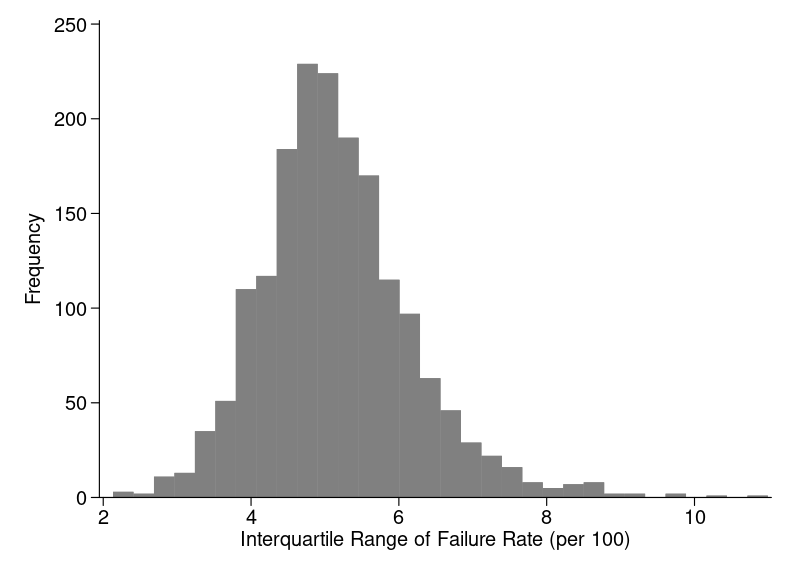
\includegraphics[width=\linewidth,height=0.66\textheight,keepaspectratio]{results/figures/desc/Failure_IQR_1_1_0.png}}%
      \only<2>{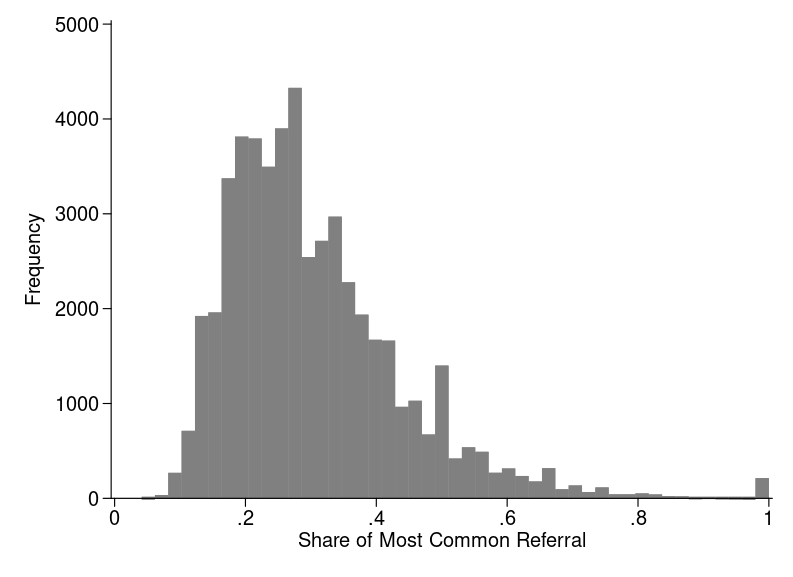
\includegraphics[width=\linewidth,height=0.66\textheight,keepaspectratio]{results/figures/desc/HighestShare_1_1_0.png}}%
      \only<3>{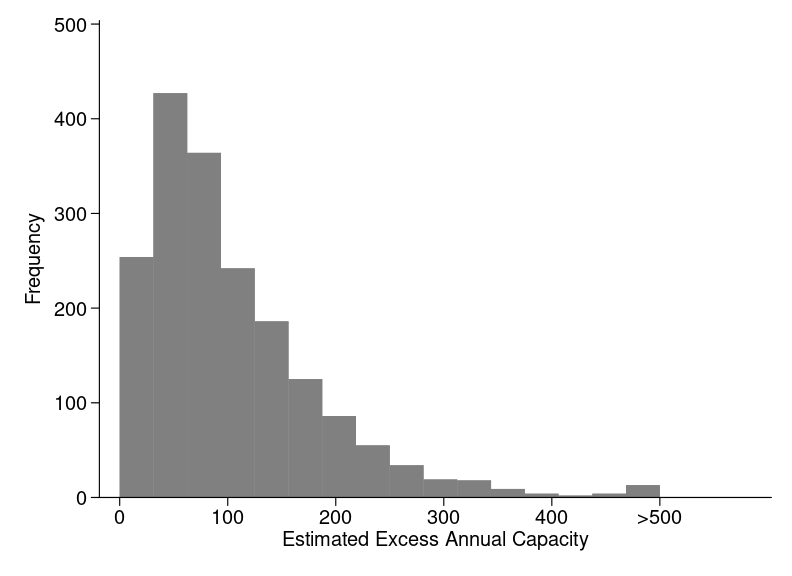
\includegraphics[width=\linewidth,height=0.66\textheight,keepaspectratio]{results/figures/desc/Excess_Capacity.png}}
  \end{columns}
\end{frame}

%% ═══════════════════════════════════════════════════════════════
%% DESIGN-BASED EVIDENCE
%% ═══════════════════════════════════════════════════════════════

\section{Do PCPs Respond to Bad Outcomes?}
\sectionframe

\begin{frame}{PCPs refer less to a surgeon after their own patient has a bad outcome}
  \begin{columns}[c,onlytextwidth]
    \column{0.42\textwidth}
      \small
      \begin{itemize}\setlength{\itemsep}{7pt}
        \item Every referral is an event; the outcome is whether the PCP's \emph{next} referral goes to the same surgeon
        \item Failures against successes, with surgeon-by-year fixed effects and the pair's prior history
        \item A failure lowers the chance of returning by \rereferPct{}\% (\rereferFX{} on a base of \rereferBase{}), unchanged with PCP fixed effects
        \item Largest where the PCP knows the surgeon least: \rereferPcthistzero{}\% at a first referral, \rereferPcthisttwo{}\% after five or more
      \end{itemize}
    \column{0.55\textwidth}
      \centering
      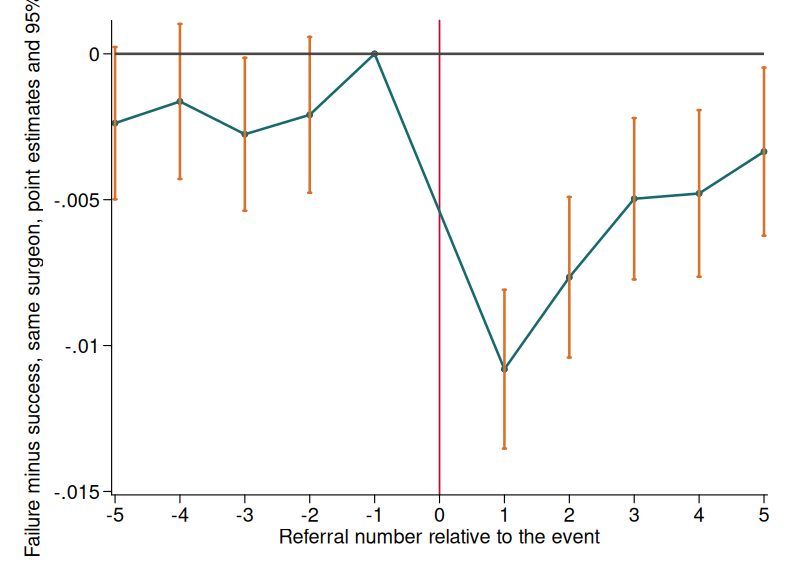
\includegraphics[width=\linewidth,height=0.66\textheight,keepaspectratio]{results/figures/rf/Rereferral_EventStudy_1_1_0.png}\\
      {\scriptsize\color{emoryMid}Event study in referral order, failure minus success windows}
  \end{columns}
\end{frame}

%% ═══════════════════════════════════════════════════════════════
%% MODEL
%% ═══════════════════════════════════════════════════════════════

% Model, stepped: the utility one term at a time, then learning, behavior, estimation
\section{A Learning Model of Referrals}
\sectionframe

\begin{frame}<1-9>[t]{PCPs learn about surgeon quality from their own patients' outcomes}
  \vspace{0.1cm}
  \hspace*{-0.2cm}\begin{tikzpicture}[
      eq/.style={font=\large, inner sep=2pt},
      box/.style={rounded corners=3pt, line width=0.9pt, inner sep=4pt},
      card/.style={rounded corners=3pt, line width=0.7pt, text width=2.05cm, align=center,
                   font=\scriptsize, inner sep=4pt, anchor=north},
      panel/.style={rounded corners=4pt, line width=0.7pt, draw=emoryRule, fill=emoryLight,
                    text width=4.0cm, align=left, font=\scriptsize, inner sep=6pt, anchor=north,
                    execute at begin node={\hyphenpenalty=10000 \exhyphenpenalty=10000}}]
    \node[eq] at (0.55,0) {$U_{ijt} =$};
    \node[eq] (q)  at (2.35,0)  {$\alpha\, m_{ijt}$};
    \node[eq] at (3.55,0) {$+$};
    \node[eq] (x)  at (4.65,0)  {$\pi\, x_{ijt}$};
    \node[eq] at (5.8,0) {$+$};
    \node[eq] (f)  at (6.95,0)  {$f(e_{ijt})$};
    \node[eq] at (8.1,0) {$+$};
    \node[eq] (c)  at (9.25,0)  {$\gamma\, n_{jt}$};
    \node[eq] at (10.4,0) {$+$};
    \node[eq] (xi) at (11.55,0) {$\xi_j$};
    \node[eq] at (12.85,0) {$+\ \epsilon_{ijt}$};
    \only<2->{\draw[box, draw=emoryBlue, fill=emoryBlue, fill opacity=0.08] (q.south west) rectangle (q.north east);
      \draw[emoryBlue, line width=0.7pt] (q.south) -- (2.35,-0.75);
      \node[card, draw=emoryBlue, fill=emoryBlue!6, text=emoryBlue] at (2.35,-0.75)
        {belief about quality, with weight $\alpha$};}
    \only<3->{\draw[box, draw=emoryMid, fill=emoryMid, fill opacity=0.08] (x.south west) rectangle (x.north east);
      \draw[emoryMid, line width=0.7pt] (x.south) -- (4.65,-0.75);
      \node[card, draw=emoryMid, fill=emoryMid!6, text=emoryDark] at (4.65,-0.75)
        {distance to the surgeon};}
    \only<4->{\draw[box, draw=emoryGold, fill=emoryGold, fill opacity=0.10] (f.south west) rectangle (f.north east);
      \draw[emoryGold, line width=0.7pt] (f.south) -- (6.95,-0.75);
      \node[card, draw=emoryGold, fill=emoryGold!8, text=emoryGold!60!black] at (6.95,-0.75)
        {familiarity: past referrals to $j$};}
    \only<5->{\draw[box, draw=emoryMid, fill=emoryMid, fill opacity=0.08] (c.south west) rectangle (c.north east);
      \draw[emoryMid, line width=0.7pt] (c.south) -- (9.25,-0.75);
      \node[card, draw=emoryMid, fill=emoryMid!6, text=emoryDark] at (9.25,-0.75)
        {congestion: the surgeon's other patients};}
    \only<6->{\draw[box, draw=emoryMid, fill=emoryMid, fill opacity=0.08] (xi.south west) rectangle (xi.north east);
      \draw[emoryMid, line width=0.7pt] (xi.south) -- (11.55,-0.75);
      \node[card, draw=emoryMid, fill=emoryMid!6, text=emoryDark] at (11.55,-0.75)
        {surgeon fixed effect};}
    \only<7->{\node[panel] at (2.3,-2.6) {%
      {\footnotesize\bfseries\color{emoryBlue}Learning}\\[3pt]
      Beliefs start from a common beta prior and update with each patient's outcome\\[3pt]
      $\displaystyle m_{ijt} = \frac{\rho\eta + \text{past successes}}{\eta + \text{past referrals}}$\\[3pt]
      $\rho$ = prior mean, $\eta$ = prior strength};}
    \only<8->{\node[panel] at (6.95,-2.6) {%
      {\footnotesize\bfseries\color{emoryBlue}Behavior}\\[3pt]
      Myopic PCPs refer on current beliefs\\[3pt]
      Forward-looking PCPs also value what a referral teaches them, through a Gittins index};}
    \only<9->{\node[panel] at (11.6,-2.6) {%
      {\footnotesize\bfseries\color{emoryBlue}Estimation}\\[3pt]
      Logit in each of 306 HRRs\\[3pt]
      Congestion by 2SLS, distance-based instrument\\[3pt]
      $\rho$ = market success rate, $\eta$ = 1 or 5};}
  \end{tikzpicture}
\end{frame}

\begin{frame}{Identification in one slide}
  The belief term splits into the prior and the past success rate, $\bar y$:
  $$\alpha\, m_{ijt} = \alpha\,\frac{\rho\eta}{\eta + e_{ijt}} + \alpha\,\frac{e_{ijt}}{\eta + e_{ijt}}\,\bar y_{ijt}$$
  \begin{itemize}\setlength{\itemsep}{7pt}
    \item $\alpha$: a PCP with many past patients at two surgeons but different success rates; as $e \to \infty$ the belief term is $\alpha \bar y$
    \item $\eta$: how fast the effect of the success rate grows with the number of past patients; weakly identified, so fixed at 1 or 5
    \item Familiarity $f(e)$: the effect of past referrals that remains once the belief term is accounted for
    \item Congestion $\gamma$: surgeon-by-period fixed effects, then 2SLS with volume predicted from \emph{other} patients' distances
  \end{itemize}
\end{frame}

%% ═══════════════════════════════════════════════════════════════
%% RESULTS
%% ═══════════════════════════════════════════════════════════════

\begin{frame}{Estimates}
  \begin{center}
  \small
  \begin{tabular}{lcccccc}
    \toprule
    & & \multicolumn{5}{c}{Percentile across HRRs} \\
    \cmidrule(lr){3-7}
    Myopic model & Mean & 10th & 25th & 50th & 75th & 90th \\
    \midrule
    $\alpha$ ($\eta = 1$) & 0.202 & 0.000 & 0.000 & 0.117 & 0.283 & 0.537 \\
    $\alpha$ ($\eta = 5$) & 0.397 & 0.000 & 0.000 & 0.212 & 0.561 & 1.089 \\
    $\pi$ (distance, per mile) & $-0.069$ & $-0.099$ & $-0.082$ & $-0.068$ & $-0.053$ & $-0.038$ \\
    \bottomrule
  \end{tabular}
  \end{center}
  \vspace{0.1cm}
  \begin{itemize}\setlength{\itemsep}{5pt}
    \item $\alpha/\pi$: a success is worth about \alphaDistRatioMyopic{} miles of travel, in line with small quality elasticities elsewhere
    \item Familiarity is large and rising: 1.1 after one past patient, 2.4 after eight to ten
    \item Congestion: 100 more patients over three years lowers the referral probability by 7--9\%
    \item Forward-looking model: $\alpha$ somewhat larger (0.26 at $\eta = 1$), everything else the same
  \end{itemize}
\end{frame}

% Results, stepped: estimates, full information, quality weighted like distance
\section{Counterfactuals}
\sectionframe

\begin{frame}<1-5>[t]{What we find}
  \vspace{0.2cm}
  \begin{tikzpicture}[
      res/.style={rounded corners=4pt, line width=0.7pt, draw=emoryRule, fill=emoryLight,
                  text width=5.6cm, minimum height=3.8cm, align=left, inner sep=7pt, anchor=north west, font=\footnotesize,
                  execute at begin node={\hyphenpenalty=10000 \exhyphenpenalty=10000}},
      done/.style={anchor=west, inner sep=0pt, font=\footnotesize}]
    \path[use as bounding box] (0,0.2) rectangle (13.6,-5.8);
    \only<2->{\node[done] at (0,0) {\makebox[1.8cm][l]{\bfseries\color{emoryGold}0 to 2 pp}{\color{emoryDark}PCPs weigh quality lightly relative to other factors}};}
    \only<3->{\node[done] at (0,-0.4) {\makebox[1.8cm][l]{\bfseries\color{emoryGold}23\%}{\color{emoryDark}reallocated under full information with existing relationships, failures fall by \healthFXMeanCurrentEtaFiveMyopic{} per 100}};}
    \only<4->{\node[done] at (0,-0.8) {\makebox[1.8cm][l]{\bfseries\color{emoryGold}32\%}{\color{emoryDark}reallocated when the relationships are reset, with no health gain}};}
    \only<5>{\node[done] at (0,-1.2) {\makebox[1.8cm][l]{\bfseries\color{emoryGold}20\%}{\color{emoryDark}of failures avoided when quality counts like distance}};}
    \only<5>{\node[res, text width=10.0cm, minimum height=0pt, font=\small, anchor=north] at (6.8,-2.1) {%
      {\bfseries\color{emoryBlue}Takeaway\par}\vspace{2pt}
      \begin{itemize}\setlength{\itemsep}{3pt}
        \item The gains from quality information alone are bounded by the small weight PCPs place on quality, and they depend on the referral relationships PCPs already have
        \item Tools that raise that weight could deliver substantially larger health improvements
        \item The same under the forward-looking model (\reallocationMeanCurrentEtaFiveFWD{}\% and \reallocationMeanFWD{}\% reallocated, failures \healthFXMeanCurrentEtaFiveFWD{} and \healthFXMeanFWD{} per 100)
      \end{itemize}\vspace{-14pt}};}
    \only<1>{\node[res] at (0,-1.2) {%
      {\small\bfseries\color{emoryBlue}PCPs weigh quality lightly relative to other factors\par}\vspace{2pt}
      {\LARGE\bfseries\color{emoryGold}0 to 2 pp\par}\vspace{4pt}
      drop in referral probability after one more failure, across markets. Where PCPs respond, the average is \partialFXNonzeroMyopic{} pp.\par};}
    \only<2>{\node[res] at (0,-1.2) {%
      {\small\bfseries\color{emoryBlue}Full information\par}\vspace{2pt}
      {\LARGE\bfseries\color{emoryGold}\reallocationMeanCurrentEtaFiveMyopic{}\%\par}\vspace{4pt}
      of patients go to a different surgeon when PCPs know true quality and keep their existing relationships. Failures fall by \healthFXMeanCurrentEtaFiveMyopic{} per 100, with gains in most markets\par};}
    \only<3>{\node[res] at (0,-1.2) {%
      {\small\bfseries\color{emoryBlue}Existing relationships are with better surgeons\par}\vspace{2pt}
      {\LARGE\bfseries\color{emoryGold}\reallocationMeanMyopic{}\%\par}\vspace{4pt}
      of patients move under full information when the relationships are reset, with no health gain\par\vspace{4pt}
      Success rates rise with relationship length, so familiarity has already sorted PCPs toward better surgeons\par};}
    \only<4>{\node[res] at (0,-1.2) {%
      {\small\bfseries\color{emoryBlue}Quality weighted like distance\par}\vspace{2pt}
      {\LARGE\bfseries\color{emoryGold}20\%\par}\vspace{4pt}
      of failures avoided when one SD of quality counts as much as one SD of distance\par\vspace{4pt}
      150 to 200 more successes per 10,000, still subject to distance and surgeon capacity\par};}
    \node[anchor=north] at (10.15,-1.2) {%
      \only<1>{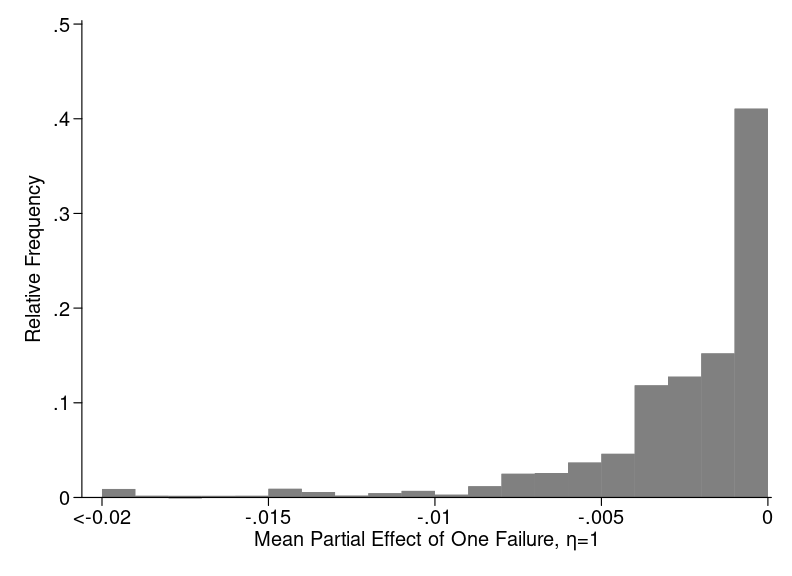
\includegraphics[width=6.6cm,height=4.5cm,keepaspectratio]{results/figures/myopic-timevary/Mean_Partial_FX_Failure_Myopic_eta1.png}}%
      \only<2>{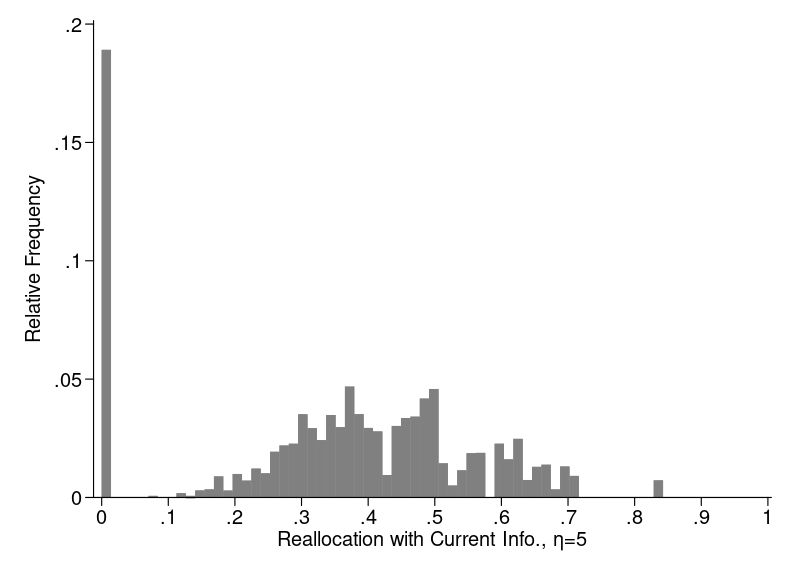
\includegraphics[width=6.6cm,height=4.5cm,keepaspectratio]{results/figures/myopic-timevary/Reallocation_Current_Myopic_eta5.png}}%
      \only<3>{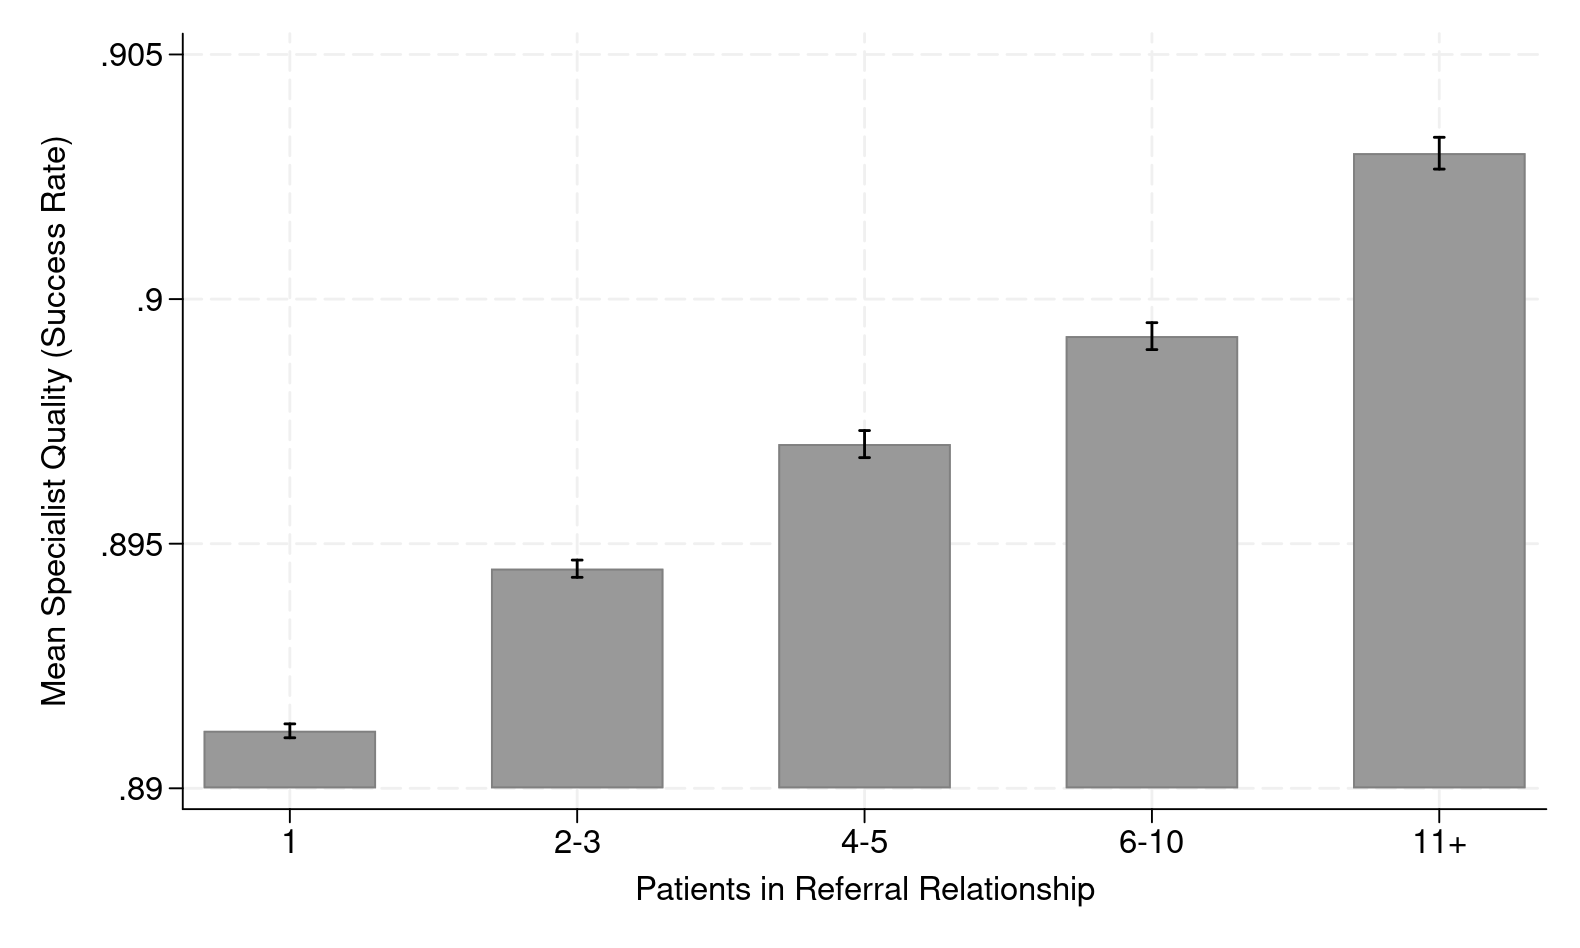
\includegraphics[width=6.6cm,height=4.5cm,keepaspectratio]{results/figures/Familiarity_Quality_Patients_1_1_0.png}}%
      \only<4>{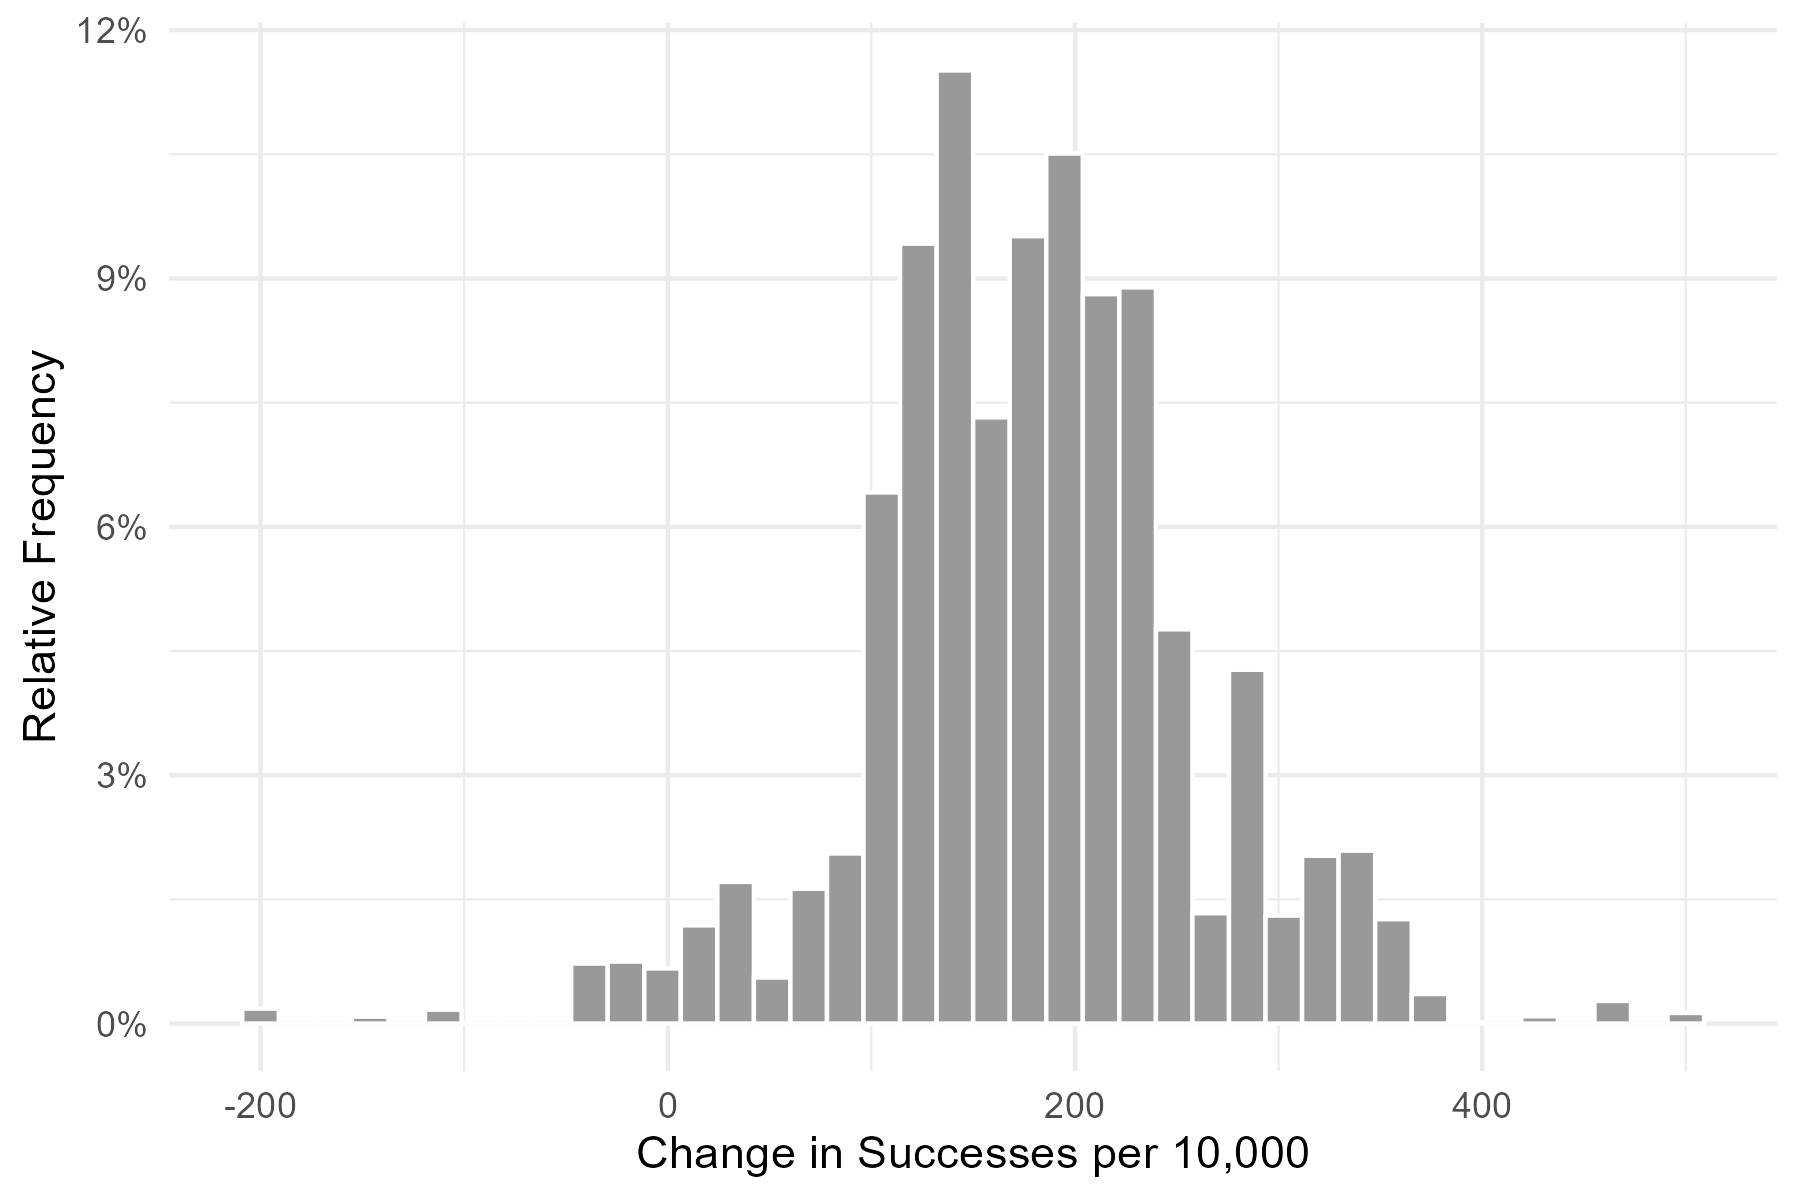
\includegraphics[width=6.6cm,height=4.5cm,keepaspectratio]{results/figures/myopic-timevary/Mean_Health_FX_qualmax_amatch_Myopic_eta1.png}}};
  \end{tikzpicture}
\end{frame}
\begin{frame}{Summary}
  \begin{itemize}\setlength{\itemsep}{10pt}
    \item Surgeon quality varies widely within markets, and PCPs respond to their own patients' outcomes, most when they know the surgeon least
    \item A structural learning model of referrals with habit persistence and capacity constraints puts a small weight on quality: a success is worth about \alphaDistRatioMyopic{} miles
    \item Full information reallocates about a quarter of referrals with small but meaningful health gains, and the gains depend on the referral relationships PCPs already have
    \item Quality information works best alongside existing referral relationships rather than in place of them
  \end{itemize}
  \vspace{0.3cm}
  {\small\color{emoryMid}ian.mccarthy@emory.edu}
\end{frame}

%% ═══════════════════════════════════════════════════════════════
%% BACKUP
%% ═══════════════════════════════════════════════════════════════

\section{Backup}
\sectionframe

\begin{frame}[noframenumbering]{Re-referral design}
  \small
  \begin{itemize}\setlength{\itemsep}{3pt}
    \item For the referral of patient $t$ from PCP $i$ to surgeon $j$, with outcome $Y_{ijt}$ and prior history $e_{ijt}$, the outcome is $R_{ijt'} = 1$ if the PCP's next patient $t'$ goes to $j$:
    $$R_{ijt'} = \gamma_{j,y(t)} + \beta (1-Y_{ijt}) + \sum_{h=1}^{5} \kappa_h \mathbf{1}\left(\min(e_{ijt},5)=h\right) + \varepsilon_{ijt}$$
    \item \rereferEvents{} referrals, \rereferFailures{} failures; $\hat\beta = \rereferFX{}$ (s.e.~\rereferSE{}); standard errors clustered by surgeon and by PCP
    \item Event study in referral order: a window is the PCP's five referrals before and after a given referral; failure windows have their only failure at position 0, success windows none
    $$R_{ijt} = \mu_{ij} + \lambda_{j y, t} + \phi_{i, t} + \sum_{k \neq -1} \delta_k \mathbf{1}(t=k) (1-Y_{ij0}) + \varepsilon_{ijt}$$
    \item First referral after a failure: \rereferESFirst{} (s.e.~\rereferESFirstSE{}) on a base of \rereferESBase{}; the gap lasts through the third referral and fades by the fifth
  \end{itemize}
\end{frame}

\begin{frame}[noframenumbering]{Setting the priors}
  \begin{itemize}\setlength{\itemsep}{9pt}
    \item Prior mean $\rho = a_0/(a_0+b_0)$ equals the market's average success rate (about 0.90), as in Coscelli and Shum (2004), Crawford and Shum (2005), and Dickstein (2018)
    \item Prior strength $\eta = a_0 + b_0$ acts like a number of patients seen before the first real one
      \begin{itemize}
        \item The likelihood is flat in $\eta$ in simulations, so it is fixed at 1 or 5; the cross-partial that identifies it moves only from 0.033 to 0.056 as $\eta$ goes from 1 to 20
        \item PCPs refer about \meanRefsPerPCP{} patients a year, so these values bracket a sensible range
        \item Other estimates and the counterfactuals are similar at both values; $\alpha$ scales with $\eta$
      \end{itemize}
  \end{itemize}
\end{frame}

\begin{frame}[noframenumbering]{Congestion stands in for surgeon capacity}
  \begin{itemize}\setlength{\itemsep}{8pt}
    \item $\gamma\, n_{jt}$: a surgeon treating more patients is less attractive for the next one (for example, wait times)
    \item Two steps (Richards-Shubik, Roberts and Donohue 2022, following Bayer and Timmins 2007)
      \begin{itemize}
        \item Estimate the logit with a surgeon-by-period fixed effect $\delta_{j\tau} = \gamma n_{j\tau} + \xi_j$
        \item Regress $\hat\delta_{j\tau}$ on $n_{j\tau}$ by 2SLS
      \end{itemize}
    \item Instrument: the surgeon's patient count predicted from distances alone; other patients' distances shift the surgeon's volume but not this patient's referral (first-stage F above 1,000)
    \item In the counterfactuals, volumes and referrals are re-solved together as a fixed point
  \end{itemize}
\end{frame}

\begin{frame}[noframenumbering]{Forward-looking PCPs also value experimentation}
  \begin{itemize}\setlength{\itemsep}{8pt}
    \item Myopic: refer to the surgeon with the highest expected payoff for this patient
    \item Forward-looking: also value what the referral teaches about the surgeon, for future patients
      \begin{itemize}
        \item Gittins index $g(m, v)$, rising in the variance of beliefs, with the closed-form approximation of Brezzi and Lai (2002)
        \item No parameters beyond the myopic model
      \end{itemize}
    \item The forward-looking $\alpha$ is somewhat larger (0.26 vs.\ 0.20 at $\eta = 1$); counterfactual results are similar in the two versions
  \end{itemize}
\end{frame}

\begin{frame}<1-4>[t,noframenumbering]{Risk adjustment changes little}
  \vspace{0.2cm}
  \begin{tikzpicture}
    \path[use as bounding box] (0,0.3) rectangle (13.6,-5.4);
    \node[anchor=base east, inner sep=0pt, font=\footnotesize\bfseries, text=emoryMid] at (13.4,0) {Mean $\hat\alpha$};
    \rrow{-0.7}{1-}{Baseline}{0.192}
    \rrow{-1.35}{2-}{Restrict to DRG 470}{0.216}
    \rsub{-1.6}{2-}{Joint replacement without major complications, 86\% of cases}
    \rrow{-2.4}{3-}{Use risk-adjusted surgeon quality}{0.192}
    \rsub{-2.65}{3-}{Observed minus expected failures, with expected failures from age, sex, race, DRG, and the Charlson index}
    \rsub{-3.45}{3-}{Correlation with raw quality is 0.84}
    \rcard{4}{The estimated weight on quality is stable.}
  \end{tikzpicture}
\end{frame}

\begin{frame}[noframenumbering]{Full information: distributions across markets (myopic, $\eta = 1$)}
  \scriptsize
  \centering
  \begin{tabular}{@{}l@{\hspace{3pt}}c@{\hspace{3pt}}c@{}}
    & Share reallocated & Change in success probability \\
    \raisebox{0.38in}{Existing} &
    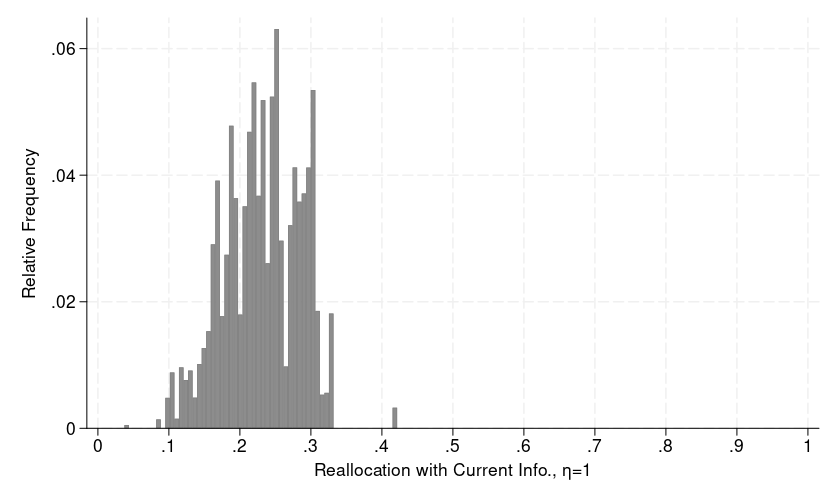
\includegraphics[width=0.41\textwidth,height=1.05in,keepaspectratio]{results/figures/myopic-timevary/Reallocation_Current_Myopic_eta1.png} &
    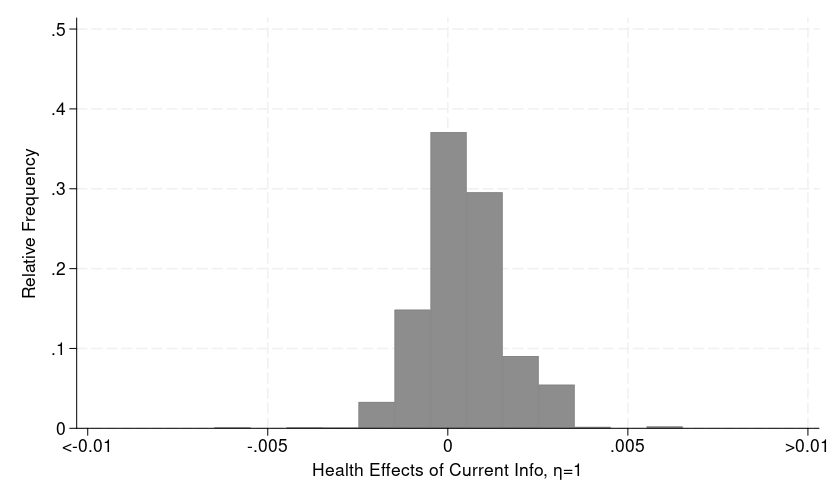
\includegraphics[width=0.41\textwidth,height=1.05in,keepaspectratio]{results/figures/myopic-timevary/Mean_Health_FX_Current_Myopic_eta1.png} \\
    \raisebox{0.38in}{Reset} &
    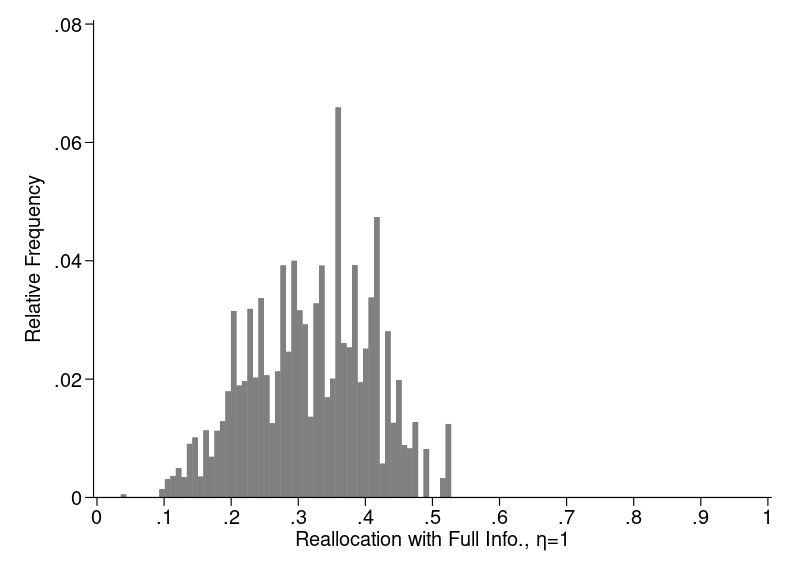
\includegraphics[width=0.41\textwidth,height=1.05in,keepaspectratio]{results/figures/myopic-timevary/Reallocation_Full_Myopic_eta1.png} &
    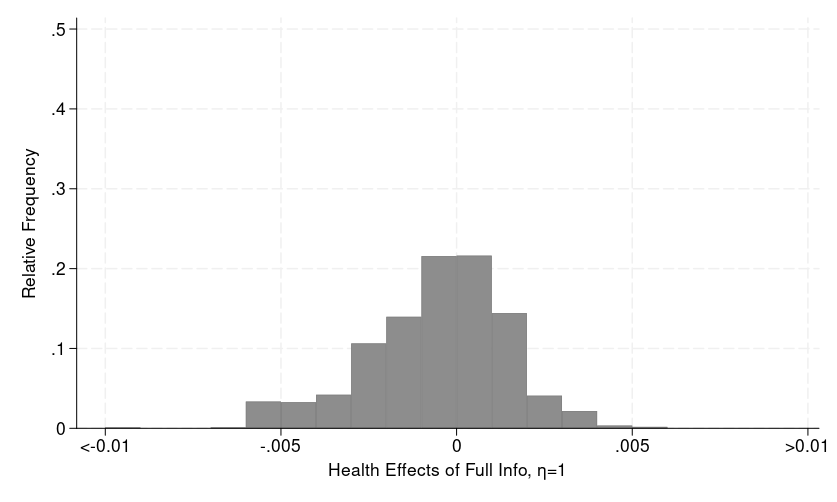
\includegraphics[width=0.41\textwidth,height=1.05in,keepaspectratio]{results/figures/myopic-timevary/Mean_Health_FX_Full_Myopic_eta1.png}
  \end{tabular}
\end{frame}

\end{document}
